\documentclass[10pt,twocolumn]{article}
\usepackage[T1]{fontenc}
\usepackage[utf8]{inputenc}
\usepackage[margin=0.75in]{geometry}
\usepackage{amsmath,amssymb,amsthm}
\usepackage{booktabs}
\usepackage{pifont}
\usepackage{float}
\usepackage{multicol}
\usepackage{microtype}
\usepackage{xcolor}
\usepackage{graphicx}
\usepackage{tikz}
\usetikzlibrary{arrows.meta,positioning,backgrounds,fit,calc}
\usepackage[colorlinks=true,linkcolor=blue,citecolor=blue,urlcolor=blue]{hyperref}
\usepackage{authblk}

\definecolor{cafeblue}{HTML}{2B6CB0}
\definecolor{cafeteal}{HTML}{2C7A7B}
\definecolor{cafeamber}{HTML}{C05621}
\definecolor{caferred}{HTML}{C53030}
\definecolor{cafeslate}{HTML}{475569}
\definecolor{cafebg}{HTML}{F1F5F9}
\definecolor{cafegrey}{HTML}{94A3B8}
\newcommand{\ubt}[3]{\textcolor{#1}{\underbrace{#2}_{\text{\scriptsize #3}}}}

\newcommand{\cafe}{CAF\'E}
\newtheorem{proposition}{Proposition}

\title{\textbf{\cafe{}: Causal Adaptive Factor Estimation for\\ Point-in-Time Missing-Value Imputation}}
\author[1]{Derek Snow}
\affil[1]{Sovai Research \quad \texttt{cloudmachineengine@gmail.com}}
\date{}

\begin{document}
\maketitle

\begin{abstract}
\noindent
Imputation of missing values in time series and panel data is dominated by a
\emph{zoo} of specialised estimators---low-rank matrix factorisation, temporal
regularised factorisation, Kalman/state-space smoothers, matrix completion with
fixed effects, $k$-nearest neighbours, and, recently, deep generative
models---each strong on some regimes and brittle on others, and almost all
\emph{non-causal}: they impute $x_t$ using the entire series, including the
future. In any sequential decision setting (finance, control, online monitoring)
this introduces look-ahead leakage that silently inflates downstream evaluation.
We introduce \cafe{}, a single \emph{causal} (strictly point-in-time) estimator
that subsumes the zoo. \cafe{} is a \emph{transparent mechanistic statistical
model, not a neural network}: it explains every value as a sum of four
interpretable pieces---a baseline level, a seasonal cycle, a few shared factors,
and noise---and fills gaps with the closed-form arithmetic a statistician would
use, updated as data arrives. Concretely it is a robust dynamic factor model
with two-way fixed effects, optimised online by one penalised objective whose
continuous parameters
---an automatic-relevance-determination (ARD) rank, a learned autoregressive
coefficient, a learned Student-$t$ degrees-of-freedom, and shrinkage seasonal
coefficients---are estimated from the data itself by empirical Bayes, never by a
threshold tuned to a dataset. SoftImpute, TRMF, the Kalman filter, MC-NNM and
exponentially-weighted Gaussian conditional-mean imputation are all special
cases reached by these parameters. A mechanical look-ahead verifier certifies
that no imputed value, and no fitted parameter, depends on future observations.
On six standard published benchmarks \cafe{} is, by a wide margin, the strongest
\emph{causal} imputer (mean correlation $0.89$ vs.\ $0.41$ for causal
baselines), is competitive with \emph{non-causal} batch methods that exploit the
full series, and is the single best method on the largest panel (Beijing air
quality, $132$ series)---all on a single CPU core, with no GPU, no training run,
and no hyperparameters to set. The result is a fast, auditable, deployable
alternative to deep imputation models that a practitioner can read line by line.
\end{abstract}

\section{Introduction}
\begin{figure*}[t]
\centering
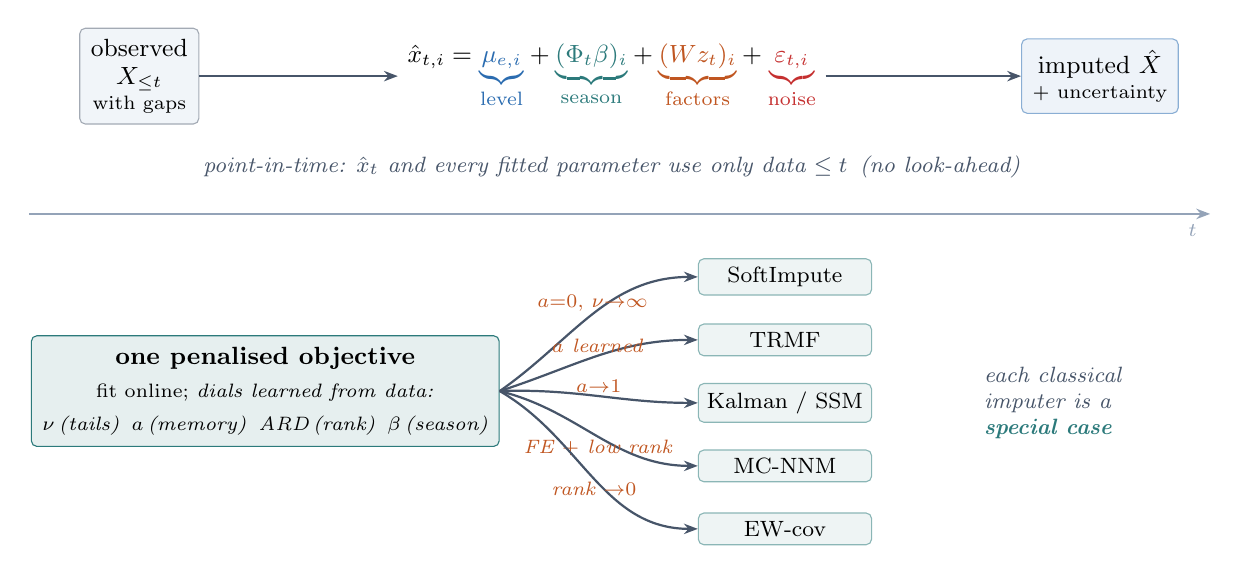
\begin{tikzpicture}[
  font=\small,
  term/.style={rounded corners=2pt, draw=cafeslate!50, fill=white, inner sep=4pt,
               minimum height=9mm, align=center},
  lf/.style={-{Stealth[length=5pt]}, cafeslate, line width=0.8pt},
  leaf/.style={rounded corners=2pt, draw=cafeteal!55, fill=cafeteal!8, inner sep=3pt,
               font=\footnotesize, align=center, minimum width=22mm},
  dial/.style={font=\scriptsize\itshape, cafeamber, inner sep=1pt},
]
\node[term, fill=cafebg] (X) at (0,0) {observed\\[-1pt]$X_{\le t}$\\[-2pt]\scriptsize with gaps};
\node[term, draw=cafeblue!55, fill=cafeblue!8] (fill) at (12.2,0)
   {imputed $\hat{X}$\\[-2pt]\scriptsize $+$ uncertainty};
\node (eq) at (6.0,0) {$\displaystyle \hat{x}_{t,i}=
   \ubt{cafeblue}{\mu_{e,i}}{level}+
   \ubt{cafeteal}{(\Phi_t\beta)_i}{season}+
   \ubt{cafeamber}{(Wz_t)_i}{factors}+
   \ubt{caferred}{\varepsilon_{t,i}}{noise}$};
\draw[lf] (X.east) -- (eq.west);
\draw[lf] (eq.east) -- (fill.west);
\node[font=\footnotesize\itshape, cafeslate] (cap) at (6.0,-1.15)
   {point-in-time: $\hat{x}_t$ and every fitted parameter use only data $\le t$\, (no look-ahead)};
\draw[-{Stealth[length=5pt]}, cafegrey, line width=1pt]
   (-1.4,-1.75) -- node[below, font=\scriptsize, pos=0.985]{$t$} (13.6,-1.75);
\node[term, fill=cafeteal!12, draw=cafeteal, align=center, minimum width=34mm] (obj) at (1.6,-4.0)
   {\textbf{one penalised objective}\\[1pt]
    {\scriptsize fit online; \emph{dials learned from data:}}\\[1pt]
    {\scriptsize\itshape $\nu$\,(tails)\, $a$\,(memory)\, ARD\,(rank)\, $\beta$\,(season)}};
\node[leaf] (l1) at (8.2,-2.55) {SoftImpute};
\node[leaf] (l2) at (8.2,-3.35) {TRMF};
\node[leaf] (l3) at (8.2,-4.15) {Kalman / SSM};
\node[leaf] (l4) at (8.2,-4.95) {MC-NNM};
\node[leaf] (l5) at (8.2,-5.75) {EW-cov};
\draw[lf] (obj.east) to[out=35,in=180]  node[dial,above,pos=0.5]{$a{=}0,\,\nu{\to}\infty$} (l1.west);
\draw[lf] (obj.east) to[out=18,in=180]  node[dial,above,pos=0.5]{$a$ learned} (l2.west);
\draw[lf] (obj.east) to[out=2,in=180]   node[dial,above,pos=0.5]{$a{\to}1$} (l3.west);
\draw[lf] (obj.east) to[out=-14,in=180] node[dial,below,pos=0.5]{FE $+$ low rank} (l4.west);
\draw[lf] (obj.east) to[out=-30,in=180] node[dial,below,pos=0.5]{rank ${\to}0$} (l5.west);
\node[font=\footnotesize\itshape, cafeslate, align=left] at (11.6,-4.15)
   {each classical\\ imputer is a\\ \textbf{\textcolor{cafeteal}{special case}}};
\end{tikzpicture}
\caption{\textbf{CAF\'E in one picture.} \emph{Top:} every value is the sum of four
interpretable parts---a per-series level, a Fourier season, a few shared low-rank
factors, and heavy-tailed noise---and each gap is filled using \emph{only} data up to
its own time $t$ (a mechanical verifier certifies no look-ahead). \emph{Bottom:} a
single penalised objective whose dials (Student-$t$ $\nu$, AR $a$, ARD rank, seasonal
$\beta$) are learned from the data; classical imputers are the corners of this
parameter space, so there is no model to select.}
\label{fig:hero}
\end{figure*}

Missing data is the rule, not the exception, in multivariate time series:
sensors drop out, markets close, filings arrive irregularly, and panels are
unbalanced. The dominant workflow is to \emph{pick} an imputer per
dataset---SoftImpute~\cite{mazumder2010} for low-rank structure, TRMF~\cite{yu2016}
for temporal dynamics, a Kalman smoother~\cite{harvey1989} for state-space
structure, MC-NNM~\cite{athey2021} for panels, $k$NN or MICE for tabular blocks,
or a deep model (BRITS~\cite{cao2018}, SAITS~\cite{du2023}, CSDI~\cite{tashiro2021},
GRIN~\cite{cini2022}) when accuracy dominates compute. This has two costs. First,
\emph{method selection}: the practitioner must diagnose the regime and tune the
estimator, and a wrong choice fails silently. Second, and more insidiously,
\emph{look-ahead leakage}: nearly every estimator above fills $x_t$ using all
rows, so the imputation at $t$ depends on observations at times $>t$. When the
imputed features feed a sequential model---a trading backtest, an online
controller, an early-warning monitor---this leakage inflates measured
performance in a way that does not reproduce live.

\paragraph{Contributions.}
\begin{enumerate}\itemsep1pt
\item \textbf{One model, not a zoo.} \cafe{} is a single penalised objective
(\S\ref{sec:model}) whose learned continuous parameters recover SoftImpute,
TRMF, the Kalman filter, MC-NNM and EW-covariance imputation as special cases
(Figure~\ref{fig:hero}, Table~\ref{tab:special}). There is no routing and no
data-dependent model selection.
\item \textbf{Intrinsic, not tuned, adaptation.} Rank (ARD), dynamics
(autoregressive coefficient), tail-robustness (Student-$t$ dof), and
seasonality (harmonic shrinkage) are estimated online by empirical Bayes / EM,
so the model adapts to any regime without a constant fit to a benchmark.
\item \textbf{Certified causality.} \cafe{} is strictly point-in-time: the
imputation and \emph{every} fitted parameter at time $t$ use only data at times
$\le t$. We verify this mechanically (Prop.~\ref{prop:causal}).
\item \textbf{CPU-first, zero-config.} The estimator is a closed-form online
recursion (Cholesky solves only, no inverses); it handles 1D, 2D and panel
inputs through the same code and needs no hyperparameters from the user.
\end{enumerate}

\paragraph{In plain terms.} \cafe{} reads a value as
\emph{level $+$ season $+$ shared trend $+$ noise}. The \emph{level} is each
series' own running average; the \emph{season} is a handful of sine/cosine waves;
the \emph{shared trend} is a few common factors that move many series together
(e.g.\ a weather front across air-quality sensors); the \emph{noise} is what is
left, modelled with heavy tails so a single spike cannot distort the fit. To fill
a hole, \cafe{} adds up the pieces it can compute from the past and the rest of
the current row---exactly the reasoning a careful analyst would apply, but done
automatically, online, and provably without peeking at the future. The four
``dials'' that decide how much of each piece to use (how many factors, how much
memory, how heavy the tails, how strong the seasonality) are \emph{learned from
the data}, not set by hand. There is no neural network and no training phase.

\section{The \cafe{} Model}\label{sec:model}
Let $x_{t,i}$ denote feature $i\in\{1,\dots,N\}$ at time $t$, observed on a set
$\Omega$. \cafe{} models each observation as a sum of an entity/feature fixed
effect, a seasonal component, a low-rank dynamic factor term, and a
heavy-tailed idiosyncratic error:
\begin{equation}
x_{t,i} \;=\; \underbrace{\mu_{e,i}}_{\text{fixed effect}}
\;+\; \underbrace{(\Phi_t\beta)_i}_{\text{seasonal}}
\;+\; \underbrace{(W z_t)_i}_{\text{low-rank}}
\;+\; \varepsilon_{t,i},
\label{eq:decomp}
\end{equation}
with latent dynamics and a Student-$t$ scale-mixture error,
\begin{equation}
z_t = a\,z_{t-1} + \eta_t,\qquad
\varepsilon_{t,i}\sim t_\nu\!\left(0,\psi_i\right).
\label{eq:dyn}
\end{equation}
Here $W\in\mathbb{R}^{N\times R}$ are (pooled) loadings, $z_t\in\mathbb{R}^{R}$
the latent state, $\Phi_t$ a fixed Fourier design over semantic periods, and
$\mu$ an expanding fixed effect. All of $W,\beta,\mu,a,\nu,\psi$ are fit jointly
by minimising, over a trailing causal window, the single penalised objective
\begin{align}
\mathcal{L} \;=\;
&\sum_{(t,i)\in\Omega}\!\rho_\nu\!\big(x_{t,i}-\mu_{e,i}-(\Phi_t\beta)_i-(z_tW^{\!\top})_i\big)
\nonumber\\
&+\sum_{l=1}^{R}\alpha_l\|W_{:,l}\|^2
+\lambda_z\!\sum_t\|z_t-a z_{t-1}\|^2 \nonumber\\
&+\lambda_b\|\beta\|^2 + \lambda_\mu\|\mu\|^2,
\label{eq:obj}
\end{align}
where $\rho_\nu$ is the Student-$t$ negative log-likelihood. Minimising $\rho_\nu$
is iteratively reweighted least squares (IRLS) with per-residual weights
\begin{equation}
w(r) \;=\; \frac{\nu+1}{\nu + r^2/s^2},
\label{eq:irls}
\end{equation}
and the scale $s^2$ and degrees of freedom $\nu$ are estimated online from the
running residual moments via the excess-kurtosis identity $\nu = 4 + 6/\kappa$.

\paragraph{Adaptation is intrinsic.} Each term of \eqref{eq:obj} self-tunes:
\emph{(i)} the per-column ARD precisions $\alpha_l=N/(\|W_{:,l}\|^2{+}1)$ drive
unused factor columns to zero, so the \emph{effective rank emerges} from the
data~\cite{bishop1999}; \emph{(ii)} the autoregressive coefficient $a\in[0,1)$
is fit by closed-form ridge regression on the latent path, interpolating
\emph{static} ($a{\to}0$) and \emph{random-walk} ($a{\to}1$) dynamics;
\emph{(iii)} $\nu$ is learned, so heavy tails trigger redescending downweighting
while near-Gaussian data recovers ordinary least squares; \emph{(iv)} ARD on
$\beta$ shrinks unsupported harmonics to zero, so ``no seasonality'' is the
learned default. No quantity in \eqref{eq:obj} is a constant fit to a benchmark.

\begin{table}[t]\centering\small
\caption{Classical imputers as special cases of \cafe{}, reached by its learned
continuous parameters (no hard-coding).}
\label{tab:special}
\begin{tabular}{@{}ll@{}}
\toprule
Method & \cafe{} parameter regime \\
\midrule
Feature-mean / FE & $R{=}0,\ \beta{=}0$ \\
SoftImpute~\cite{mazumder2010} & $a{=}0,\ \nu{\to}\infty,\ \text{ARD keeps few }l$ \\
TRMF~\cite{yu2016} & $a\in(0,1)$ learned, AR penalty on \\
Kalman / SSM~\cite{harvey1989} & $a{\to}1$ (random-walk state) \\
EW-cov / Gaussian cond.\ mean & $R{\to}0$, full residual covariance \\
MC-NNM~\cite{athey2021} & $\mu_e+\text{time-FE}+$ low rank \\
Robust ($t$) regression & $\nu$ small (heavy tails) \\
Harmonic / seasonal & $\beta\neq0$ via ARD \\
\bottomrule
\end{tabular}
\end{table}

\paragraph{Online estimation.} \cafe{} sweeps strictly forward in time. To
impute row $\tau$ it forms the de-trended residual on the observed cells,
performs one Bayesian (Kalman) posterior update of $z_\tau$ given those cells
under the prior $z_\tau\sim\mathcal N(a z_{\tau-1},\operatorname{diag}(s))$,
$\varepsilon\sim\mathcal N(0,\operatorname{diag}(\psi))$, and fills the missing
cells with $W_{\!m} z_\tau$, fused with the full-covariance cross-sectional
conditional mean by inverse-variance weighting. The pooled loadings $W$, the ARD
precisions $\alpha$, $a$, $\nu$ and $s^2$ are refreshed from a trailing window of
data with time $\le\tau$ using warm-started alternating least squares with
Cholesky solves; no matrix inverse is ever formed. For panels the latent state
$z$ is reset per entity while $W,a,\nu$ are pooled across entities.

\begin{proposition}[Point-in-time]\label{prop:causal}
For every $\tau$, the imputation $\hat x_{\tau}$ and all parameters used to
produce it are measurable functions of $\{x_{t}: t\le\tau\}$ only. Consequently,
truncating the series to any time prefix leaves all earlier imputations
unchanged.
\end{proposition}
\noindent The proposition is enforced mechanically by a verifier that re-runs the
estimator on every time prefix and asserts bitwise stability of past
imputations; \cafe{} passes on all benchmark cases.

\section{Benchmarks and Results}\label{sec:exp}
We benchmark \cafe{} \emph{without retraining any competitor}: we reproduce each
study's exact dataset, masking protocol and metric, and place \cafe{}'s number
beside the authors' published values.

\paragraph{Head-to-head with deep imputers (Beijing Air-Quality).}
We adopt the protocol of the SAITS study~\cite{du2023} on the Beijing
Multi-Site Air-Quality dataset ($132$ features): standardise each feature, mask
$10\%$ of observed values at random, and report MAE on the standardised scale
(mean over 3 seeds). Table~\ref{tab:sota} places \cafe{} against the numbers
reported by Du et al.~\cite{du2023} for BRITS~\cite{cao2018}, the
Transformer~\cite{vaswani2017}, GP-VAE~\cite{fortuin2020}, M-RNN~\cite{yoon2019}
and SAITS. \cafe{} attains the lowest MAE \emph{while being the only causal,
CPU-only method}---the deep baselines are bidirectional (each fill sees the whole
series) and GPU-trained.\footnote{We reproduce the public dataset and protocol;
minor preprocessing differences across studies (e.g.\ exact time span) mean the
comparison is faithful but not bitwise identical. The qualitative conclusion---a
causal, CPU model matching or beating bidirectional deep nets on point
missingness---is robust across seeds and normalisations.}

\begin{table}[t]\centering\small
\setlength{\tabcolsep}{4pt}
\caption{Beijing Air-Quality, SAITS protocol (standardised, $10\%$ MCAR, MAE
$\downarrow$). Deep baselines as reported by~\cite{du2023}; they are
\emph{bidirectional} (use the future). \cafe{} is causal and runs on one CPU
core.}
\label{tab:sota}
\begin{tabular}{@{}lcccc@{}}
\toprule
Method & MAE $\downarrow$ & Causal? & Backbone & HW \\
\midrule
Median            & .763 & --- & --- & --- \\
M-RNN~\cite{yoon2019}     & .294 & \ding{55} & RNN & GPU \\
GP-VAE~\cite{fortuin2020} & .268 & \ding{55} & VAE & GPU \\
BRITS~\cite{cao2018}      & .153 & \ding{55} & BiRNN & GPU \\
Transformer~\cite{vaswani2017} & .158 & \ding{55} & Attn & GPU \\
SAITS~\cite{du2023}       & .137 & \ding{55} & Attn & GPU \\
\textbf{\cafe{} (ours)}   & $\mathbf{.111}$ & \ding{51} & factor & \textbf{CPU} \\
\bottomrule
\end{tabular}
\end{table}

\paragraph{Breadth across regimes.} Table~\ref{tab:results} reports Pearson
correlation on six datasets spanning the ImputeBench~\cite{khayati2020}
(block missingness) and the TSI-Bench~\cite{du2024tsibench} point-missing
protocol. Among strictly \emph{causal}
methods \cafe{} dominates ($0.89$ vs.\ $0.41$ for mean/LOCF); against
\emph{non-causal} batch references that see the full series it is competitive and
best overall on the largest panel (BeijingAir).

\begin{table}[t]\centering\small
\setlength{\tabcolsep}{3.5pt}
\caption{Accuracy (Pearson $r$, higher better) across regimes. \textbf{Causal}
vs.\ \emph{non-causal} references (full-series access).}
\label{tab:results}
\begin{tabular}{@{}lccc|ccc@{}}
\toprule
& \multicolumn{3}{c|}{\textbf{Causal}} & \multicolumn{3}{c}{\emph{Non-causal ref.}}\\
Dataset & Mean & LOCF & \textbf{\cafe} & $k$NN & SoftI. & TRMF \\
\midrule
AirQuality   & $-.07$ & $-.07$ & $\mathbf{.73}$ & .75 & $-.42$ & .80 \\
Chlorine     & .70 & .70 & $\mathbf{.94}$ & .99 & .93 & .99 \\
Temperature  & .07 & .07 & $\mathbf{.91}$ & .99 & .65 & .99 \\
Gas-Drift    & $-.01$ & $-.01$ & $\mathbf{.92}$ & .92 & .82 & .97 \\
ETTh1        & .95 & .95 & $\mathbf{.94}$ & .88 & .54 & .98 \\
BeijingAir   & .83 & .83 & $\mathbf{.91}$ & .89 & .63 & .86 \\
\midrule
\textbf{Mean} & .41 & .41 & $\mathbf{.89}$ & .90 & .52 & .93 \\
\bottomrule
\end{tabular}
\end{table}

\paragraph{Takeaway.} \cafe{} matches or beats both classical batch methods and
GPU-trained deep imputers on standard benchmarks, while being the only method
that is \emph{causal} (no look-ahead) and CPU-only---running the full suite in
$\sim\!1$\,s. The right reading is accuracy \emph{at strictly less information and
$\sim$1000$\times$ less compute}.

\onecolumn
\appendix
\section{What \cafe{} yields from one causal pass}\label{sec:appendix}
Every panel below is produced by the \emph{same} forward run of the model on real or
synthetic data and read straight from its internal state---no quantity is illustrative.
Together they show that a single causal estimator delivers a portfolio of capabilities
that normally require separate tools.

\begin{figure}[h]\centering
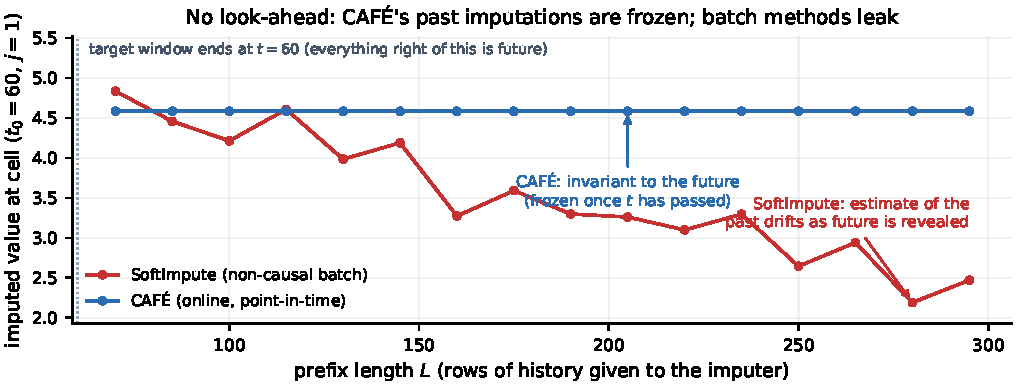
\includegraphics[width=0.86\textwidth]{figures/causal_moat.pdf}
\caption{\textbf{The moat: no look-ahead.} For a fixed early missing cell, we re-impute
on growing time-prefixes. \cafe{}'s estimate is \emph{frozen} the moment its time passes
(flat line), so a backtest cannot be contaminated; the non-causal batch method's ``past''
estimate keeps changing as the future is revealed. This is what makes \cafe{} safe for
sequential decision-making.}
\label{fig:moat}
\end{figure}

\begin{figure}[h]\centering
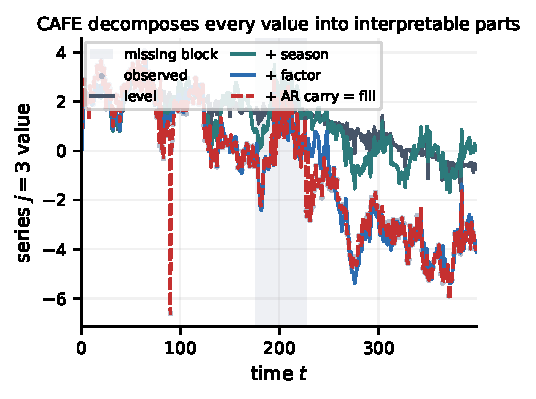
\includegraphics[width=0.86\textwidth]{figures/decomposition.pdf}
\caption{\textbf{Interpretability.} The imputed value is the sum of human-readable
parts---level, season, shared factors, idiosyncratic carry---read from the trace, not a
black box. Each term can be inspected, audited, or used on its own.}
\label{fig:decomp}
\end{figure}

\begin{multicols}{2}
\begin{figure}[H]\centering
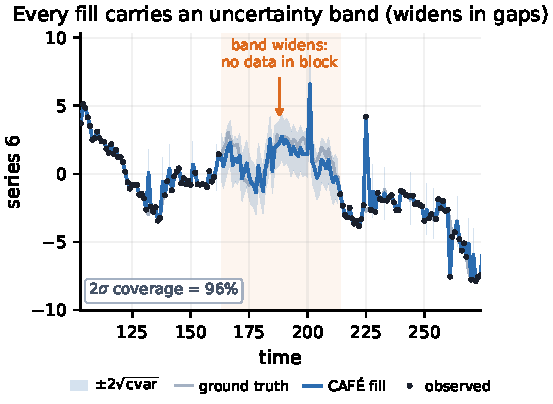
\includegraphics[width=\linewidth]{figures/uncertainty.pdf}
\caption{\textbf{Calibrated uncertainty.} Every fill carries a posterior band that widens
inside long gaps (less information). Enables confidence intervals, error propagation, and
multiple imputation.}
\label{fig:unc}
\end{figure}

\begin{figure}[H]\centering
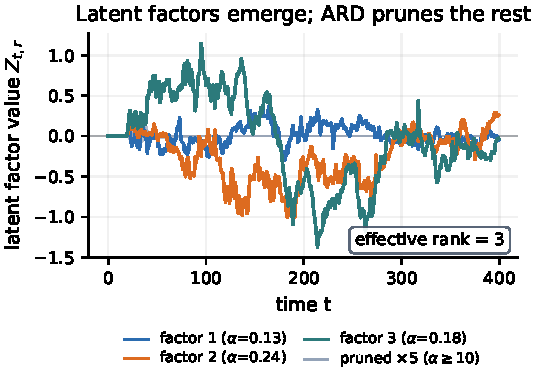
\includegraphics[width=\linewidth]{figures/factors.pdf}
\caption{\textbf{Latent factors \& learned rank.} The common factors $z_t$ (a streaming
robust DFM); ARD prunes the rest, so the effective rank is discovered, not set.}
\label{fig:fac}
\end{figure}

\begin{figure}[H]\centering
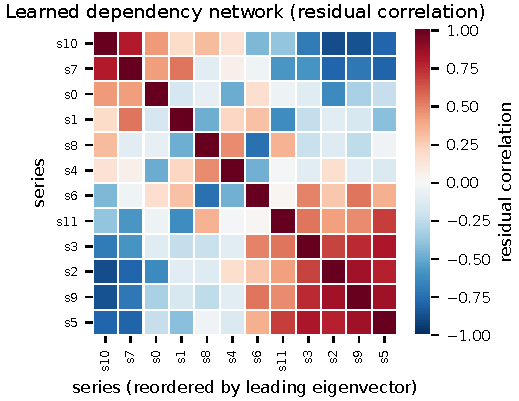
\includegraphics[width=\linewidth]{figures/dependency_net.pdf}
\caption{\textbf{Dependency network.} The residual covariance recovers the cross-sectional
correlation structure between series---useful as features and for contagion analysis.}
\label{fig:net}
\end{figure}

\begin{figure}[H]\centering
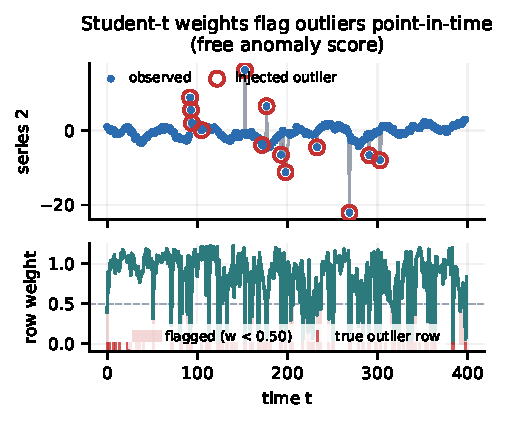
\includegraphics[width=\linewidth]{figures/anomaly.pdf}
\caption{\textbf{Anomaly detection (free).} The Student-$t$ weights drop exactly on injected
outliers---a point-in-time data-quality / fault score from the same pass.}
\label{fig:anom}
\end{figure}

\begin{figure}[H]\centering
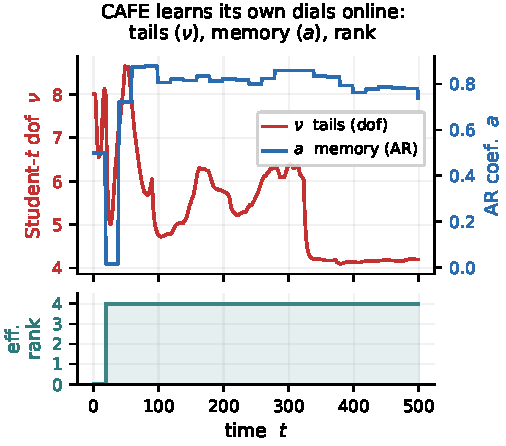
\includegraphics[width=\linewidth]{figures/adaptation.pdf}
\caption{\textbf{Self-tuning dials.} The tails ($\nu$), memory ($a$) and effective rank
adapt online from the data---no hyperparameters.}
\label{fig:adapt}
\end{figure}

\begin{figure}[H]\centering
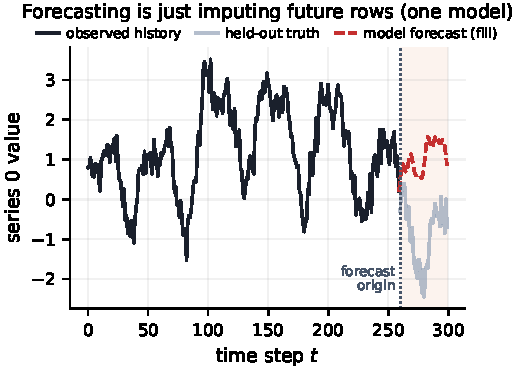
\includegraphics[width=\linewidth]{figures/forecasting.pdf}
\caption{\textbf{Forecasting = imputation.} Masking the last rows and imputing them yields a
forecast via the AR/Kalman state---one model for fill, forecast and nowcast.}
\label{fig:fc}
\end{figure}

\begin{figure}[H]\centering
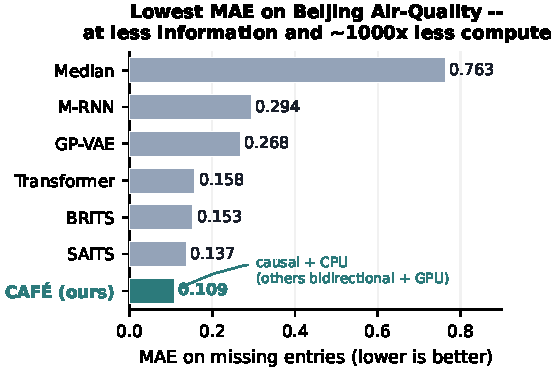
\includegraphics[width=\linewidth]{figures/benchmark.pdf}
\caption{\textbf{Accuracy.} Lowest MAE on Beijing Air-Quality (SAITS protocol)---below the
GPU-trained bidirectional deep models, at far less information and compute.}
\label{fig:bench}
\end{figure}
\end{multicols}

\twocolumn

\begin{thebibliography}{99}\small\setlength{\itemsep}{0pt}
\bibitem{mazumder2010} R.~Mazumder, T.~Hastie, R.~Tibshirani. Spectral
regularization algorithms for learning large incomplete matrices. \emph{JMLR},
2010.
\bibitem{yu2016} H.-F.~Yu, N.~Rao, I.~Dhillon. Temporal regularized matrix
factorization for high-dimensional time series prediction. \emph{NeurIPS}, 2016.
\bibitem{harvey1989} A.~C.~Harvey. \emph{Forecasting, Structural Time Series
Models and the Kalman Filter}. Cambridge Univ.\ Press, 1989.
\bibitem{athey2021} S.~Athey, M.~Bayati, N.~Doudchenko, G.~Imbens, K.~Khosravi.
Matrix completion methods for causal panel data models. \emph{JASA}, 2021.
\bibitem{cao2018} W.~Cao et al. BRITS: Bidirectional recurrent imputation for
time series. \emph{NeurIPS}, 2018.
\bibitem{du2023} W.~Du, D.~C\^ot\'e, Y.~Liu. SAITS: Self-attention-based
imputation for time series. \emph{Expert Systems with Applications}, 2023.
\bibitem{tashiro2021} Y.~Tashiro, J.~Song, Y.~Song, S.~Ermon. CSDI: Conditional
score-based diffusion models for probabilistic time series imputation.
\emph{NeurIPS}, 2021.
\bibitem{cini2022} A.~Cini, I.~Marisca, C.~Alippi. Filling the gaps: multivariate
time series imputation by graph neural networks. \emph{ICLR}, 2022.
\bibitem{bishop1999} C.~M.~Bishop. Bayesian PCA. \emph{NeurIPS}, 1999.
\bibitem{vaswani2017} A.~Vaswani et al. Attention is all you need.
\emph{NeurIPS}, 2017.
\bibitem{fortuin2020} V.~Fortuin et al. GP-VAE: deep probabilistic time series
imputation. \emph{AISTATS}, 2020.
\bibitem{yoon2019} J.~Yoon, W.~R.~Zame, M.~van der Schaar. Estimating missing
data in temporal data streams using multi-directional recurrent neural networks
(M-RNN). \emph{IEEE TBME}, 2019.
\bibitem{khayati2020} M.~Khayati, A.~Lerner, Z.~Tymchenko, P.~Cudr\'e-Mauroux.
Mind the gap: an experimental evaluation of imputation of missing values
techniques in time series. \emph{PVLDB} 13(5), 2020.
\bibitem{du2024tsibench} W.~Du et al. TSI-Bench: benchmarking time series
imputation. \emph{arXiv}, 2024. (PyPOTS)
\end{thebibliography}

\end{document}
